\documentclass[conference]{IEEEtran}
\IEEEoverridecommandlockouts
% The preceding line is only needed to identify funding in the first footnote. If that is unneeded, please comment it out.
\include{pythonlisting}
\usepackage{cite}
\usepackage{amsmath,amssymb,amsfonts}
\usepackage{algorithmic}
\usepackage[ruled,vlined]{algorithm2e}

\usepackage{hyperref}

\usepackage{graphicx}
\usepackage{textcomp}
\usepackage{url}
\usepackage{xcolor}
\def\BibTeX{{\rm B\kern-.05em{\sc i\kern-.025em b}\kern-.08em
    T\kern-.1667em\lower.7ex\hbox{E}\kern-.125emX}}
\begin{document}

\title{Exploring numerical calculations with CalcNet}

\author{\IEEEauthorblockN{Ashish Rana}
\IEEEauthorblockA{ Thapar Institute of Engg. and Tech. India\\
arana\_be15@thapar.edu}
\and
\IEEEauthorblockN{Avleen Malhi}
\IEEEauthorblockA{Aalto University Finland\\
avleen.malhi@aalto.fi}
}


\maketitle

\begin{abstract}

Neural networks are not great generalizers outside their training range i.e. they are good at capturing bias but might miss the overall concept. Important issues with neural networks is that when testing data goes outside training range they fail to predict accurate results. Hence, they loose the ability to generalize a concept. For systematic numeric exploration neural accumulators (NAC) and neural arithmetic logic unit(NALU) are proposed which performs excellent for simple arithmetic operations. But, major limitation with these units is that they can't handle complex mathematical operations \& equations. For example, NALU can predict accurate results for multiplication operation but not for factorial function which is essentially composition of multiplication operations only. It is unable to comprehend pattern behind an expression when composition of operations are involved.
Hence, we propose a new neural network structure effectively which takes in complex compositional mathematical operations and produces best possible results with small NALU based neural networks as its pluggable modules which evaluates these expression at unitary level in a bottom-up manner. We call this effective neural network as CalcNet, as it helps in predicting accurate calculations for complex numerical expressions even for values that are out of training range. As part of our study we applied this network on numerically approximating complex equations, evaluating biquadratic equations and tested reusability of these modules. We arrived at far better generalizations for complex arithmetic extrapolation tasks as compare to both only NALU layer based neural networks and simple feed forward neural networks. Also, we achieved even better results for our golden ratio based modified NAC and NALU structures for both interpolating and extrapolating tasks in all evaluation experiments.Finally, from reusability standpoint this model
demonstrate strong invariance for making predictions on different tasks.

\end{abstract}


\section{Introduction}

Generalization of concepts is the fundamental component while defining intelligence in a system  \cite{b1} \cite{b2}. While, neural networks can be applied on numerical quantities they are not associated with generalization capabilities \cite{b3, b4}. We define generalization capabilities as the ability to understand complex numerical expressions that identifies compositional patterns. 
Meaning that a neural network should understand all the operations in an expression and predict high accuracy results for unseen and out of training range data.
Failure to understand these numeric generalizations is clearly visible in Table \ref{tab:table1} when test range lies outside the training range even for simpler target functions. This highlights hard memory commit behavior of the biases learnt by neural networks instead of learning abstract concepts. For mitigating this problem of memorizing behavior in neural networks, special numerically biased modules known as Neural accumulators (NAC) and neural arithmetic logic units (NALU) \cite{b5} were introduced. These units have performed exceptionally well for generalization on simple numerical operators and have achieved state-of-the-art results. But, again these units fail to make generalizations for complex mathematical equations as these units only learns the simple mathematical operations only with their weights being biased specially towards -1, 0, 1. In Figure \ref{fig1} and its weight matrices analysis, we see addition and subtraction being modelled with such numerical biases. Only meaning, biased values around -1, 0, 1 gets better results for numeric computations. Also, Figure \ref{fig2} highlights this biased nature for NAC units which helps this unit to model these functions and for NALU also, scaling up and down mechanisms for multiplication and division operations is highlighted ever increasing approximate curve specified for larger values in Figure \ref{fig2}.

\begin{figure}[!h]
\centering
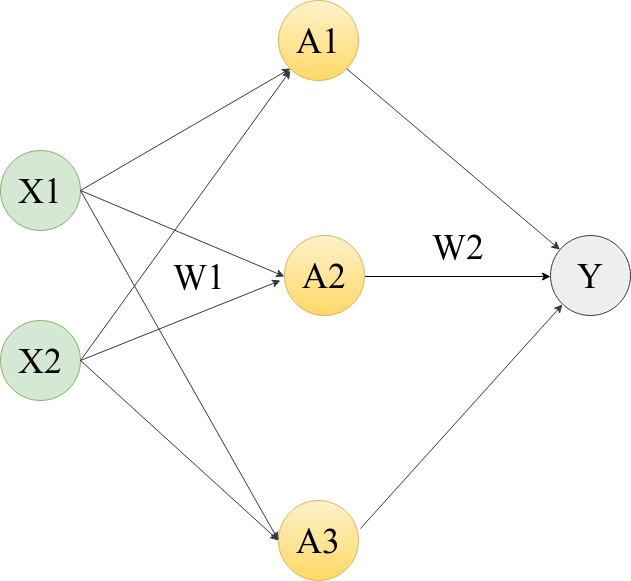
\includegraphics[width=0.18\textwidth]{_assets/NeuralMLP.png}
\caption{Simple MLP with W$_1$, W$_2$ weight matrices with Y as output for X$_1$, X$_2$ as inputs. For modelling addition and subtraction operations follow along with below mentioned W$_1$, W$_2$ values. No bias vector \textit{b} assumed for this MLP and only linear activations considered.}
\label{fig1}
\end{figure}

\begin{itemize}
\item For modelling addition operation Y=X$_1$+X$_2$, W$_1$ and W$_2$ can have possible following arrangement of values.
\[
\begin{bmatrix}
    1  &  0      \\
    1  &  1      \\
    0  &  1
\end{bmatrix}
,
\begin{bmatrix}
    1        \\
    0  		 \\
    1      
\end{bmatrix} 
\]

\item For modelling subtraction operation Y=X$_1$-X$_2$, W$_1$ and W$_2$ can again be created with only [-1, 0, 1] values with slightly  different arrangement. Hence, restricting weights to these values added numerical bias which is better for arithmetic calculation related tasks.
\[
\begin{bmatrix}
    1  &  0      \\
    1  &  1      \\
    0  &  1
\end{bmatrix}
,
\begin{bmatrix}
    1        \\
    0  		 \\
    -1      
\end{bmatrix} 
\]

\end{itemize}

\begin{figure}[!h]
\centering
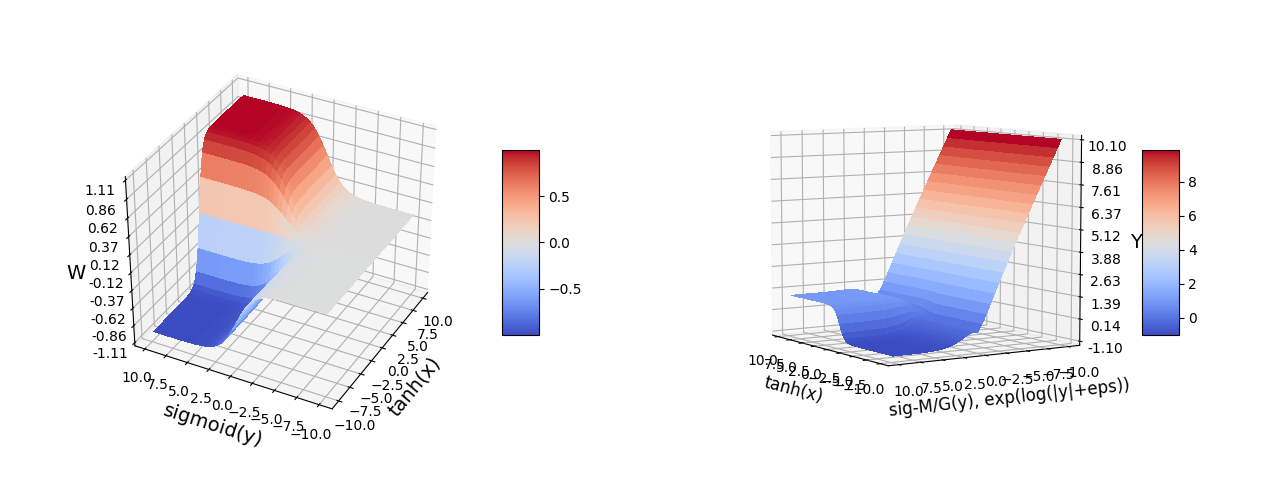
\includegraphics[width=0.50\textwidth]{_assets/NAC&NALU.png}
\caption{\textbf{\textit{Left: }}NAC is biased with learning [1, 0, 1] values i.e. it either accumulate or deduct instead of scaling, perfect for addition \& subtraction operations.
\textbf{\textit{Right: }}Approximate curve for NALU focuses on scaling up and down nature along with superimposition of [1, 0, 1] bias from NAC which is relatively better for multiply, divison \& power functions. }
\label{fig2}
\end{figure}

NALU units can't handle negative targets as exponential space only gives positive values which adds some limitations to it, shown in Figure \ref{fig2}. Along, with that these units can't breakdown common complex functions like factorial, exponential etc. which are essentially formed from repeated multiplication operations. Hence, we need an architecture that can comprehend such functions and breakdown their complexity into simplest most unary or binary operations along with considering sign of targets.

In this paper, we introduce a new neural network architecture pipeline which is effectively feed forward in nature that can perform complex calculations by utilizing NAC and NALU MLPs as its fundamental unit and a parser algorithm for breaking down numeric calculations into their lower most granularity operations. It achieves state of the art results for numerical computations and manipulations for complex arithmetic expressions with our golden ratio based NAC and NALU units. Hence, creating neural networks that truly understands numerical manipulations which can have feasible practical applications. Like, quantum mechanics equations involving uncertainity because of duality in particles for example, heisenberg uncertainty equation that giving approximated position or momentum of a particle. The proposed network can simulate this approximation behavior with the formulated algorithm. Finally, we applied and tested our effective neural network architecture on biquadratic formula equations. This experiment also tested robustness and invariance of this network as trained models from different numerical equation's data were reutilized.



\section{Related Work}

Very deep neural networks have performed extremely well for computer vision tasks \cite{b6} and reducing computations for such networks \cite{b9}. But, basic quantitative manipulation \& reasoning is also very important. These conceptions by our brain is extensively studied task in \cite{b1, b2, b10}. 

For encouraging further systematic numerical extrapolation, a new architecture known as a neural arithmetic logic unit (NALU) is proposed which helps in representing numerical quantities in the form of linear activations allowing manipulations by employing primitive arithmetic operators which are being restrained by learned gates \cite{b5}. The NALU enhanced neural networks are able to count objects in images, execute computer code, translate numerical language into real-valued scalars, perform arithmetic over images of numbers, track time. It obtains consequential generalizations within and outside the training range of the numerical values allowing magnitude orders beyond numerical training ranges compared to conventional architectures. Another neural networks based assessment method was proposed using NALU where weight determination is done through training \cite{b13}. The obtained scores from pseudo-subjective assessment are being compared with the actual values stored in the database. Normally, neural network (NN) based prediction tool's accuracy needs to be tested beyond the NN weight training set. Nonetheless, insistent residual errors were further down-scaled by employing particle swarm optimization which is NN weights post-processing for improving the accuracy. This assessment has considerable applications for long term evolution (LTE) network operators Quality-of-Experience-aware network optimization.

Neural networks have successfully learned to represent numerical quantities and manipulate them with proper learning biases. But, still this behavior doesn't highlight systematic generalizations \cite{b3, b4}. However, in nature beings and animal species have shown numerical extrapolation capabilities \cite{b10, b11} implying that numerical manipulation is ecologically advantageous. Hence, creating networks with true numerical manipulation power showcase intelligence for developing smart systems.
Our solution models and manipulate mathematical symbols with semantic sense of mathematical grammar used while parsing the numeric expression.
Currently, our approach uses precedence rules to evaluate the mathematical expressions with respect to different operators. We haven't explored training neural networks for learning precedence logic for mathematical operators used as a part of this study.

\section{CalcNet}

Neural networks have shown great deal of success from computer vision \cite{b6, b10}, text and audio analysis \cite{b7}, to reinforcement learning \cite{b8}. But, real world problems involving numerical analysis where theory and applied science merges is still quite unexplored with neural networks. Exploring networks learning numerical manipulation based on sequence learning is not the aim of this paper. Instead, our work focuses on increasing generalization capabilities i.e. better predictions by the network for extrapolating results onto unseen solution space as well for observing underlying structure of governing-equations \cite{b12}. For this we propose a simple feed forward effective neural network architecture that have the ability to parse complex mathematical expressions with NAC and NALU multilayer perceptrons(MLPs) as it fundamental units for making predictions. This network is having NAC and NALU layers which handles each operator from given complex mathematical equation separately.
The expression evaluation follows the order of precedence rule while parsing as defined in regular mathematics for these operators. After each module has evaluated the higher precedence sub-expression their output goes in as input to find output of another lower precedence order sub-expression. This process goes on till the complete expression is evaluated as highlighted in CalcNet infix expression evaluation algorithm stated below. The net error produced by this model is the summation of error produced by each of it's modules. Intuitively stating, the errors get traversed onto other neural network modules and gets accumulated producing even more wrong predictions in later stages of expression evaluation. Here, Figure \ref{fig3} highlights the workings of this effective neural architecture, explains error propagation and presents the equivalent functioning architecture of this network.
We have also introduced modifications to NAC and NALU units and have achieved even better results for simple arithmetic operations and complex equation solving tasks by replacing expontential value($\textbf{\textit{e}}$) in \textit{sigmoid} and \textit{tanh} with golden ratio($\phi$). These variants are represented as  G-NAC and G-NALU respectively where \textit{G} signifies their golden ratio base instead of an exponential one.  

\begin{figure}[!h]
\centering
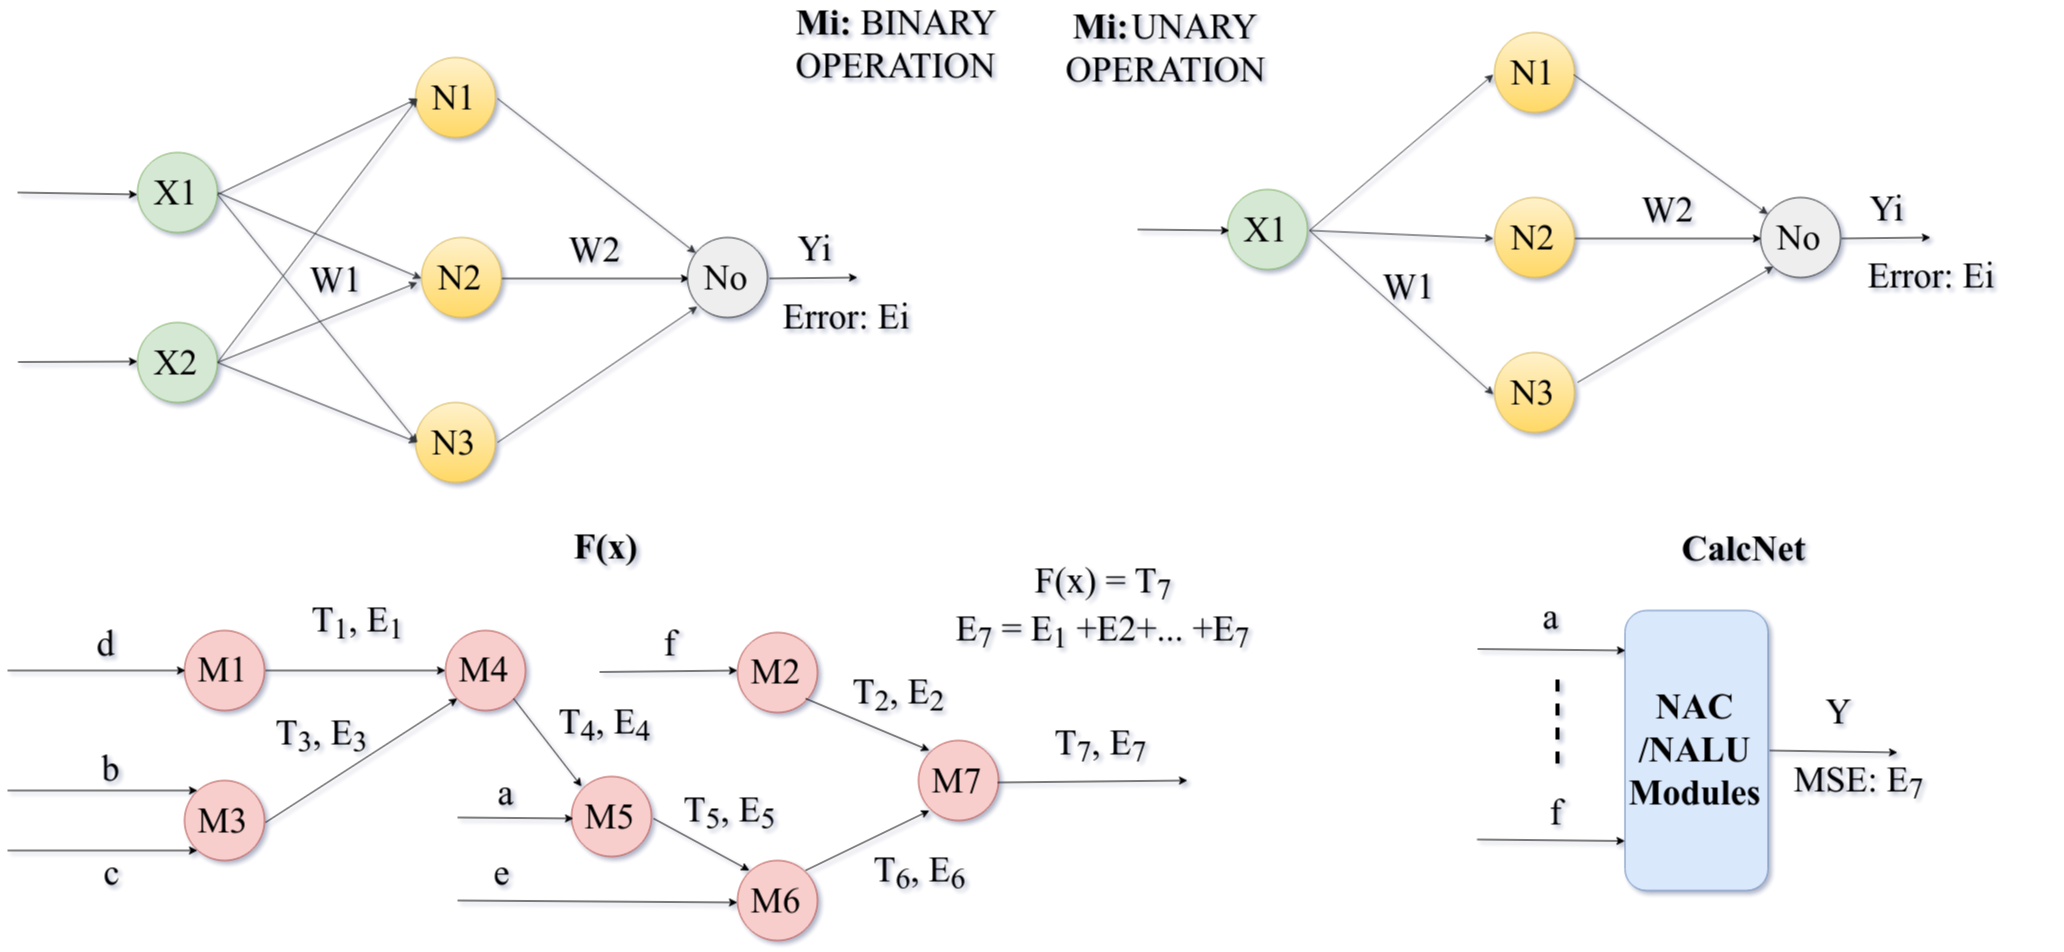
\includegraphics[width=0.51\textwidth]{_assets/CalcNet.png}
\caption{\textbf{\textit{Top-Left: }}NAC/NALU based MLP module for binary operator.
\textbf{\textit{Top-Right: }}NAC/NALU based MLP module for unary operator. 
\textbf{\textit{Bottom-Left: }} For f(x)=a+b/c*$\sqrt{d}$-e+f\textsuperscript{2} the CalcNet algorithm  proceed in the specified manner with errors propagating in additive fashion. 
\textbf{\textit{Bottom-Right: }} Shows abstract blackbox representation with any number of inputs \& operators from which output \& error information can be utilized. 
 }
\label{fig3}
\end{figure}


\begin{algorithm}
\SetAlgoLined
\textbf{Inputs:} String S$_i$, with operands and operators for \textbf{f(x)}. \\
\textbf{x$_i$:} x$_1$, x$_2$,...., x$_n$, where each \textit{x$_i$} is a variable.\\
\textbf{op$_i$:} op$_1$, op$_2$,...., op$_n$, where each \textit{op$_i$} is a variable.\\
\textbf{Pre-requisites:} \\
\textbf{M\textsubscript{NAC}:} NAC modules pre-trained for each accumulating/deducting operands, \\
\textbf{M\textsubscript{NALU}:} NALU modules pre-trained for each scaling operand \\
\textbf{Initialization:} \textbf{S\textsubscript{vr}:} variable operand stack, \textbf{S\textsubscript{op}:} operator stack \\

\KwResult{Predicted Outcome for \textbf{f(x)}}

 \While{ reading(\textit{char} from S$_i$ of \textbf{f(x)}) != None}{
  
\uIf{\textit{char} == operand}{
    \textit{push}(S\textsubscript{vr}, \textit{char})
  }
  \uElseIf{\textit{char} == operator}{
      \While{ precedOrder(top(S\textsubscript{op})) $\ge$ precedOrder(\textit{char}) }{
	  op$_i$ = pop(S\textsubscript{op}) \\
	  v$_a$ = pop(S\textsubscript{vr}) \\
	  v$_b$ = pop(S\textsubscript{vr})  \\
      // \textit{selectModule} function select ANN NAC/NALU model based on operator \\
      t$_i$ = predictCalcNet(v$_a$, v$_b$, selectModule(op)) \\
      \textit{push}(S\textsubscript{vr}, t$_i$) \\
      }
      \textit{push}(S\textsubscript{op}, t$_i$) \\

  }
  \uElseIf{\textit{char} == '('}{
  		
  	  \While{ \textit{char} == ')' }{
  	  
	  op$_i$ = pop(S\textsubscript{op}) \\
	  v$_a$ = pop(S\textsubscript{vr}) \\
	  v$_b$ = pop(S\textsubscript{vr})  \\
      t$_i$ = predictCalcNet(v$_a$, v$_b$, selectModule(op)) \\
      \textit{push}(S\textsubscript{vr}, t$_i$) \\

      }
  }
  \Else{
	return \textbf{\textit{Parse Error}}  
  }

 }
 // When no more characters are left for reading. \\
  \While{empty(pop(S\textsubscript{op})) != false}{
      op$_i$ = pop(S\textsubscript{op}) \\
 	  v$_a$ = pop(S\textsubscript{vr}) \\
	  v$_b$ = pop(S\textsubscript{vr})  \\  	  
      t$_i$ = predictCalcNet(v$_a$, v$_b$, selectModule(op)) \\
      \textit{push}(S\textsubscript{vr}, t$_i$) \\
  }
	
  \textbf{\textit{return }top(S\textsubscript{vr})}  
  
 \caption{CalcNet's Algorithm Pipeline}
\end{algorithm}

Neural accumulators (NACs) \cite{b5} supports accumulation numerically both in additive and subtractive manner. It is special type of linear layer with transformation matrix \textbf{W} being continuous and differentiable for gradient descent algorithm. Also, experiments show they exhibit better numeric bias than linear layers \cite{b5}. W = $\tanh$($\hat{W}$)$\odot$$\sigma$($\hat{M}$)  consists of elements in [-1, 1] with bias close to  −1, 0, and 1. See Figure \ref{fig2} for ideation of this concept for following equations of NAC:  a = Wx, W = $\tanh$($\hat{W}$)$\odot$$\sigma$($\hat{M}$) where \textit{$\hat{M}$}, \textit{$\hat{W}$}, are learning parameters \& \textit{W} is transformation matrix.

Also, for mathematical operations like multiply, power and division we use neural arithmetic logic units (NALUs) \cite{b5}. As visible from Figure \ref{fig2} these units are good at scaling up and down the given provided inputs. It uses weighted sum of two sub-cells, one for addition or subtraction and another of multiply, division or power functions. These units shows that neural accumulators (NACs) when extended, can learn scaling operations with gate-controlled sub-operations. See Figure \ref{fig2} for ideation of this concept with following equations for NALU: y = g$\odot$a + (1-g)$\odot$m; m = $\exp$W($\log$( $\mid$x$\mid$ + $\epsilon$)), g = $\sigma$(Gx) where \textit{m} is subcell that operates in \textit{log} space and \textit{g} is learned gate, both contains learning parameters. These units acts as fundamental tool for our numerical quantity manipulating neural network with their flat plateau like surfaces around the values -1, 0, 1 and sharp slopes to reach these values.

Numerical analysis is vast topic with lots of fields involving convergence \& series acceleration, discretization for converting continuous functions into discrete values, interpolation \& extrapolation and optimization problems, stochastic quantum equation evaluation. Our work is applicable on all approximation problems as an alternative to evaluation of complex mathematical operations i.e. we use approximating neural networks to get stochastic estimations.

\section{Experiments}

Experiments in this paper first starts with exploring performance of golden ratio based variants of NAC \& NALU modules specifically G-NAC \& G-NALU as defined earlier. We then experiment with complex arithmetic expressions testing the numeric reasoning and extrapolation capabilities of CalcNet. Finally, we used the trained modules from previous experiment to test reusability of CalcNet by evaluating all the roots of biquadratic equations from the derived formulas.

\footnote{ Experiment codes available at given github repostory url: \url{http://github.com/ashishrana160796/calcnet-experiments}}

\subsection{Golden Ratio based variants of NAC \& NALU}

Surface plots for NAC highlights clear bias towards the value -1, 0, 1 and for NALU along with these biases scaling up \& down surfaces are also superimposed. But, these sharp slopes for converging weights towards the before mentioned values might be leading to some issues with gradient propagation during the training of model with its threshold step function like logic as per our hypothesis. As per our hypothesis we do desire such biases but with regularization on sharp threshold surfaces, see Figure \ref{fig4}. Hence, to examine this we conducted experiments with modified non-linear functions having golden ratio($\phi$) as the base value instead of standard exponent($\textbf{\textit{e}}$) base for \textit{sigmoid} and \textit{tanh} functions in equations for NAC and NALU. As for comparison with vanilla NAC unit this golden ratio based NAC has less slope for more smoother transfer and update of gradient values, similar argument can be extended for NALU units, as shown in Figure \ref{fig4}.

\begin{figure}[!h]
\centering
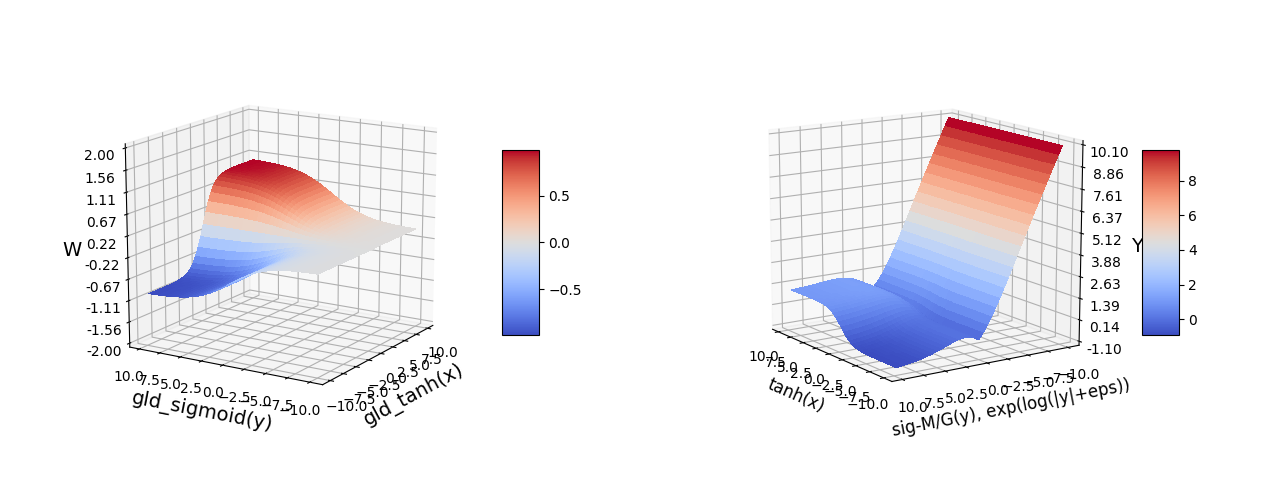
\includegraphics[width=0.50\textwidth]{_assets/GoldenNAC&NALU.png}
\caption{Golden Ratio($\phi$) based NAC \& NALU units with smoother slopes as compared to Vanilla NAC \& NALU units and lesser plateau saturation of values around [-1, 0, 1] unlike in Figure \ref{fig2}. We define our newly created units as G-NAC and G-NALU respectively where \textit{G} signifies their golden ratio base instead of an exponential one.}
\label{fig4}
\end{figure}


For this experiment, we altered the \textit{backend} script in keras source code and added our modified sigmoid \& tanh functions. We used \textit{nadam} optimizer and mean square error(\textit{MSE}) as an accuracy measure for a direct comparison with \cite{b5}. We trained NAC/NALU based model shown in Figure \ref{fig5} for 100 epoch each for 0.01, 0.001, 0.0001 learning rates respectively. The results achieved are shown in Table \ref{tab:table1} for multiple arithmetic operations. For training data, we have used 2\textsuperscript{16} data points from randomly generated distribution within the range [-10,10] for NAC and NALU modules. We haven't used negative target values for training NALUs as exponentiation operation always give positive results. Hence, signs are handled separately for multiplication, division and power operation and only magnitude is considered for training. CalcNet handles signs separately in its parsing phase instead of working with negative target values for producing better results. For interpolation task, the test data is within same range only and for extrapolation tasks we have tested our trained models on data values that are upto 5 times the training range. 

\begin{figure}[!h]
\centering
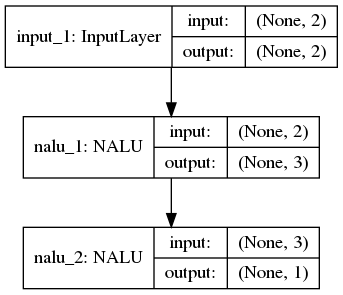
\includegraphics[width=0.24\textwidth]{_assets/model_plot.png}
\caption{MLP model with NAC/NALU units as hidden and output layers for learning static arithmetic tasks.}
\label{fig5}
\end{figure}


\bgroup
\def\arraystretch{1.5}
\begin{table}[h!]
  \begin{center}
    \caption{\textbf{Result summary for static arithmetic tasks}}
    \label{tab:table1}
    \begin{tabular}{|c|c|c|c|c|}
    
    \hline
      \textbf{Tasks} & \textbf{NAC} & \textbf{NALU} & \textbf{G-NAC} & \textbf{G-NALU}\\
    \hline    
      \multicolumn{5}{c}{\textbf{Interpolation Task: Mean Square Error Test}} \\
    \hline
      a+b & 3.601e-07 & 3.442e-05 & \textbf{1.591e-07} & 3.256e-05 \\
    \hline
      a-b & 9.065e-05 & 7.827e-04 &  \textbf{6.767e-05} & 4.033e-04\\
    \hline
      a*b & 5.2594 & 0.628 & 4.913 & \textbf{0.308} \\
    \hline
      a/b & 8.745 & 2.147 & 6.241 & \textbf{1.837} \\
    \hline
      a\textsuperscript{2} & 5.201 & 1.189 & 4.837 & \textbf{1.097}\\
    \hline
      $\sqrt{a}$ & 6.674 & 0.999 & 6.137 & \textbf{0.998}\\

    \hline    
      \multicolumn{5}{c}{\textbf{Extrapolation Task: Mean Square Error Test}} \\
    \hline
      a+b & 7.511e-06 & 9.679e-05 & \textbf{3.764e-06} & 7.809e-05 \\
    \hline
      a-b & 1.177e-04 & 9.152e-04 & \textbf{0.523e-04} & 5.148e-04 \\
    \hline
      a*b & 10.559 & 1.327 & 7.263 & \textbf{1.093} \\
    \hline
      a/b & 11.350 & 2.181 & 7.438 & \textbf{1.977} \\
    \hline
      a\textsuperscript{2} & 19.3114 & 3.246 & 16.139 & \textbf{2.830}\\
    \hline
      \textbf{$\sqrt{a}$} & 13.342 & 2.748 & 12.794 & \textbf{1.431}\\
    \hline 
    \end{tabular}
  \end{center}
\end{table}
\egroup

Our golden ratio based NAC and NALU have clearly outperformed their respective standard counterparts for every static arithmetic tasks. Golden ratio based NALU and NAC clearly highlights scope of structural improvements in existing units. Hence, our hypothesis of thresholding issues with gradient propagation for producing changes in weights does get confirmed with this experiment. Also, have used these modified units specified as G-NAC \& G-NALU for further experimentation.

\subsection{Evaluating complex expressions}

In this static arithmetic expression task we evaluated the given function \textit{f(x)} stated as, f(x)=a+b/c*$\sqrt{d}$-e+f\textsuperscript{2}. Simple MLP and also NAC/NALU based MLP won't be able to model this function for extrapolation tasks. MLP will only focus memorization of function behavior in given range and for NAC/NALU based MLP this would be too complicated numerical bias to learn. Hence, we feed this equation in to CalcNet for training where our model uses associativity and precedence rules to evaluate intermediate expressions until complete result is derived as shown below. Also, intermediate expression predictions are also stored for evaluating net ensemble error produced and relative error increase for each intermediate arithmetic operation.

\begin{itemize}
\item \textbf{Intermediate Evaluation Steps Followed:} \\
f(x) = a+b/c*$\sqrt{d}$-e+f\textsuperscript{2} \\
f(x) = a+b/c*T1-e+f\textsuperscript{2}, where T1 = $\sqrt{d}$ \\
f(x) = a+b/c*T1-e+T2, where T2 = f\textsuperscript{2} \\
f(x) = a+T3*T1-e+T2, where T3 = b/c \\
f(x) = a+T4-e+T2, where T4 = T3*T1 \\
f(x) = T5-e+T2, where T5 = a+T4 \\
f(x) = T6+T2, where T6 = T5-e \\
f(x) = T7, where T7 = T6+T2 \\

Now, for all the T\textit{i} values NAC/NALU MLP modules are trained to form an effective larger neural network which leverages associativity \& precedence grammar to form semantic relations between the intermediate expressions.
\end{itemize}

Training parameters and procedure are kept the same as earlier experiment with testing range again going upto 5 times. But, now both training and testing range are scaled by a factor of two. For training simple MLP network for comparison with CalcNet we have used linear layer as activation and for NAC/NALU based MLP same structure as Figure \ref{fig5} is used. Here, along with training the modules for each arithmetic operation they are directed to be reused for biquadratic root evaluation experiment for evaluating roots of biquadratic equation. 

\begin{itemize}
\item \textbf{Relative Error:}

Relative error metric provides a quantified measure of increase in mean square error(MSE) during prediction of outputs for particular arithmetic operation with respect to net mean square eror(MSE) for predicting the outputs.

In statistics it is formulated as:\\
\[Accuracy =\frac{\text{MSE for particular arithmetic operation}}{\text{Total MSE for all arithmetic operations}}\]
\end{itemize}

\bgroup
\def\arraystretch{1.5}
\begin{table}[h!]
  \begin{center}
    \caption{\textbf{Relative Errors for CalcNet Variants}}
    \label{tab:table2}
    \begin{tabular}{|c|c|c|c|}
    
    \hline
      \textbf{Temporary Variable} & \textbf{Evaluated Expression} & \textbf{CalcNet} & \textbf{G-CalcNet}\\
    \hline    
      \multicolumn{4}{c}{\textbf{Interpolation: Relative Error for Intermediate Steps}} \\

    \hline
	  T1  & $\sqrt{d}$ & \textbf{0.202} & 0.232 \\
	\hline	
	  T2 & f\textsuperscript{2}	& \textbf{0.234} & 0.255 \\
	\hline
	  T3 & b/c & 0.435  & \textbf{0.428}\\
	\hline
	  T4 & T3*T1  & 0.127  & \textbf{0.085}\\
	\hline
	  T5 & a+T4 &  7.188e-08  & \textbf{3.695e-08}\\
	 \hline
	  T6 & T5-e  &  4.120e-06  & \textbf{4.104e-06}\\
	 \hline
	  T7 & T6+T2 &  7.204e-08  & \textbf{3.711e-08}\\
	 \hline	  

      \multicolumn{4}{c}{\textbf{Extrapolation: Relative Error for Intermediate Steps}} \\

    \hline
	  T1  & $\sqrt{d}$ & 0.289 & \textbf{0.195}\\
	\hline	
	  T2 & f\textsuperscript{2}	& \textbf{0.341} & 0.392 \\
	\hline
	  T3 & b/c & \textbf{0.229} & 0.265 \\
	\hline
	  T4 & T3*T1  & 0.140  & \textbf{0.149}\\
	\hline
	  T5 & a+T4 &  7.891e-07 & \textbf{5.12e-07}\\
	 \hline
	  T6 & T5-e  &  1.86e-06  & \textbf{7.12e-07}\\
	 \hline
	  T7 & T6+T2 &  7.89e-07  & \textbf{5.12e-07}\\

    \hline 
    \end{tabular}
  \end{center}
\end{table}
\egroup


\bgroup
\def\arraystretch{1.5}
\begin{table}[h!]
  \begin{center}
    \caption{\textbf{Result summarization for \textit{F(x)} evaluation}}
    \label{tab:table3}
    \begin{tabular}{|c|c|c|}
    
    \hline
      \textbf{Model} & \textbf{Interpolation Task} & \textbf{Extrapolation Task}\\
    \hline
      \textbf{CalcNet} & 5.011 & 9.517 \\
    \hline
      \textbf{G-CalcNet} & \textbf{4.305} & \textbf{7.347} \\
    \hline
      \textbf{NALU-MLP} & 11.045 & 21.738 \\
    \hline
      \textbf{NAC-MLP} & 12.438 & 24.079 \\
    \hline
      \textbf{MLP} & 15.129 & 34.724 \\


    \hline 
    \end{tabular}
  \end{center}
\end{table}
\egroup

From result summarization Table \ref{tab:table3} we can clearly see our model has clearly outperformed simple MLPs and NAC/NALU MLPs for both extrapolation as well interpolation results also. Mean square error(MSE) defined in these columns for CalcNet is summation of all the errors of intermediate steps. Also, our G-NAC/G-NALU based CalcNet specified as G-CalcNet outperformed the regular CalcNet. Our results clearly shows that our models holds a semantic sense in numeric expression evaluation where as other highlights only memorization behavior. From Table \ref{tab:table2}, relative increase in error is largest for power operation followed by division for both the variants of CalcNet. Hence, even our model pipeline holds the limitations with power and division operations evaluation. 

\subsection{Evaluating biquadratic equations}

With NAC/NALU modules trained from previous experiment for CalcNet. We aim to apply our findings and results in solving real world equations. Also, we comment on the reusability of these modules in our defined model pipeline. Solutions or roots to biquadratic equations like their predecessor simpler form quadratic equations can be evaluated with formulas but these are relatively complex than evaluating simple quadratic equations. Below, we derive lucid version of formulae for $\alpha x^{4}+\beta x^{3}+\gamma x^{2}+\delta x+\varepsilon =0$ biquadratic equation. 

\begin{itemize}

\item Assuming general quartic equation of the form: $\alpha x^{4}+\beta x^{3}+\gamma x^{2}+\delta x+\varepsilon =0, \textbf{(1)}$, where x gets substituted by (y - $\beta$/4$\alpha$ ). \\
The equation is reduced to: $y^{4}+Ay^{2}+By+C=0$, \textbf{(2)}\\
with $A=\frac{\gamma }{\alpha }-\frac{3\beta ^{2}}{8\alpha ^{2}}$, \\
\\
$B=\frac{\delta }{\alpha }-\frac{\beta \gamma }{2\alpha ^{2}}+\frac{\beta^3 }{8\alpha^3 }$, \\
\\
$C=\frac{\varepsilon }{\alpha }-\frac{\beta \delta }{4\alpha ^{2}}+\frac{\beta ^{2}\gamma}{16\alpha ^{3}}-\frac{3\beta ^{4}}{256\alpha ^{4}}$. \\
After adding and subtracting $2sy^{2}+s^{2}$ to the LHS of (2) \& rearranging terms, we get: $\underset{\left( y^{2}+s\right) ^{2}}{\underbrace{y^{4}+2sy^{2}+s^{2}}}-\left[ \left( 2s-A\right) y^{2}-By+s^{2}-C\right] =0,  \textbf{(2a)}$
\\
We factorize the quadratic polynomial in \textit{2a}: $\left(2s-A\right) y^{2}-By+s^{2}-C=\left(2s-A\right)(y-y_+)(y-y_-)$ and make $y_+=y_-$ , which imposes a constraint on \textit{s}.
\\
Finally, we get: $\left( y^{2}+s+\sqrt{2s-A}y-\frac{B}{2\sqrt{2s-A}}\right)  \\
 \left( y^{2}+s-\sqrt{2s-A}y+\frac{B}{2\sqrt{2s-A}}\right)=0, \textbf{(3)}$ where \textit{s} satisfies the resolvent cubic equation as follow: $8s^{3}-4As^{2}-8Cs+\left( 4AC-B^{2}\right)=0, \textbf{(4)}$ Hence, the solution of \textbf{(2)} are solutions of \textbf{(3)}. Given by: \\

$y_{1}=-\frac{1}{2}\sqrt{2s-A}+\frac{1}{2}\sqrt{-2s-A+\frac{2B}{\sqrt{2s-A}}}$ \\
$y_{2}=-\frac{1}{2}\sqrt{2s-A}-\frac{1}{2}\sqrt{-2s-A+\frac{2B}{\sqrt{2s-A}}}$ \\
$y_{3}=\frac{1}{2}\sqrt{2s-A}+\frac{1}{2}\sqrt{-2s-A-\frac{2B}{\sqrt{2s-A}}}$ \\
$y_{4}=\frac{1}{2}\sqrt{2s-A}-\frac{1}{2}\sqrt{-2s-A-\frac{2B}{\sqrt{2s-A}}}$ \\

From this, we can get solutions for original equation. Given by: $x_{k}=y_{k}-\frac{\beta }{4\alpha },  k=1,2,3,4$

\end{itemize}

Now, with our CalcNet models we predict root for quartic equation for all \textbf{y\textit{$_i$}} values and evaluate accuracy of our models with MSE value comparison. We created test set of 2$\textsuperscript{16}$ entries with values ranging upto 5 times. Test dataset is equidistributed with values from interpolated and extrapolated values with respect to previous training range. We used previous NAC/NALU and G-NAC/G-NALU trained modules for making predictions on this testset to measure extensibility and robustness of CalcNet.

\bgroup
\def\arraystretch{1.5}
\begin{table}[h!]
  \begin{center}
    \caption{\textbf{Mean Square Error and Standard Deviations for predicting $Y_i$ values for (3)}}
    \label{tab:table4}
    \begin{tabular}{|c|c|c|}
    
    \hline
      \textbf{Root $Y_i$ values} & \textbf{CalcNet} & \textbf{G-CalcNet}\\
    \hline
      $Y_1$ & 11.324$\pm$0.53 & \textbf{8.176$\pm$0.51} \\
    \hline
      $Y_2$ & 11.861$\pm$0.58 & \textbf{8.792$\pm$0.57} \\
    \hline
      $Y_3$ & 11.506$\pm$0.56 & \textbf{8.633$\pm$0.55} \\
    \hline
      $Y_4$ & 11.137$\pm$0.62 & \textbf{8.989$\pm$0.60} \\

    \hline 
    \end{tabular}
  \end{center}
\end{table}
\egroup



G-CalcNet outperforms vanilla CalcNet in this experiment also again reconfirming our hypothesis. We achieved a good MSE error of \textbf{8.176} percent in this experiment with very low standard deviation \textbf{0.51}, refer Table \ref{tab:table4}. Hence, our model definitely is robust and can be reused again on multiple different equation with fundamental operations being the same. With the above specified accuracy and very low standard deviations, this model can be definitely used in approximation calculation methods to achieve faster results.

\section{Conclusion and Future Scope}

We were able to demonstrate higher accuracies for both interpolation and extrapolation tasks on complex arithmetic equations. Also, our modified golden ratio based G-NACs and G-NALUs structure produced better results for arithmetic operations. The algorithm governing this neural network is applicable for symbols obeying any associative grammar and precedence order. Hence, an extensible neural network module for newer domains involving new operators can be trained and re-utilized again as explained in this work.
Exploration on stochastic equation solving for quantum physics is definitely an area for future work. Further, we will explore simplification of expressions by detecting identities and theorems within the numeric expressions.

\begin{thebibliography}{00}


\bibitem{b1}  Dehaene, Stanislas. "The number sense: How the mind creates mathematics." OUP USA, 2011.
\bibitem{b2} Gallistel, C. Randy. "Finding numbers in the brain." Philosophical Transactions of the Royal Society B: Biological Sciences 373.1740 (2018): 20170119.
\bibitem{b3}Fodor, Jerry A., and Zenon W. Pylyshyn. "Connectionism and cognitive architecture: A critical analysis." Cognition 28.1-2 (1988): 3-71.
\bibitem{b4}Marcus, Gary F. "The algebraic mind: Integrating connectionism and cognitive science." MIT press, 2018.
\bibitem{b5} Trask, Andrew, et al. "Neural arithmetic logic units." Advances in Neural Information Processing Systems. 2018.

\bibitem{b6} He, Kaiming, et al. "Deep residual learning for image recognition." Proceedings of the IEEE conference on computer vision and pattern recognition. 2016.

\bibitem{b7} Lee, Younggun, et al. "Voice Imitating Text-to-Speech Neural Networks." arXiv preprint arXiv:1806.00927 (2018).

\bibitem{b8} Silver, David, et al. "Mastering Chess and Shogi by Self-Play with a General Reinforcement Learning Algorithm." arXiv preprint arXiv:1712.01815 (2017)

\bibitem{b9} He, Kaiming, et al. "Identity mappings in deep residual networks." European conference on computer vision. Springer, Cham, 2016.

\bibitem{b10} Gelman, Rochel, C. Randy Gallistel. "The child’s understanding of number." Harvard, 1978.

\bibitem{b11} Piazza, Manuela, et al. "Tuning curves for approximate numerosity in the human intraparietal sulcus." Neuron, 44:547–555, 2004.

\bibitem{b12} Brunton, Steven, et al. "Discovering governing equations from data by sparse identification of nonlinear dynamical systems." Proceedings of the National Academy of Sciences, 113(15):3932–3937, 2016.

\bibitem{b13}
Zheng, Kan, Xiaoli Zhang, Qiang Zheng, Wei Xiang, and Lajos Hanzo. "Quality-of-experience assessment and its application to video services in LTE networks." IEEE Wireless Communications 22, no. 1 (2015): 70-78.

\end{thebibliography}

\vspace{12pt}
\end{document}
